\section{Pre-Registered Exogenous News Shock Protocol and Directional Hypotheses}
\label{app-news}

This chapter specifies the experimental design testing agent reactions to unmodelled exogenous shocks. We document the five local press dispatches, the matched placebo control, the pre-registered directional sign matrix, and the longitudinal transmission mechanics.

\subsection{Experimental Conditions and Protocol Design}

The standard 21-variable survey substrate captures static individual and spatial constraints. However, real mobility choices respond continuously to unforeseen local events. We evaluate agent adaptation under two regimes: an experienced personal delay and an exogenous news dispatch read upon waking.

The news experiment exposes agents to three distinct arms across consecutive simulated days.

\textbf{Condition 1 (Nominal Reference, C1).} The agent executes standard daily routines with nominal weather and no injected press article. This arm establishes the reference modal share baseline.

\textbf{Condition 2 (Exposed Treatment, C2).} The agent reads the unedited local press dispatch during the morning waking routine, prior to selecting the first trip mode.

\textbf{Condition 3 (Placebo Control, C3).} The agent reads a neutral news dispatch matched in word count within 0.5\% to 8.0\%. The text describes a natural science discovery devoid of mobility references. This condition isolates the effect of adding textual tokens from the specific informational content of the event.

Downstream of the morning reading, the agent rates the event on a 5-point severity scale. In the evening, agents share memories across cohabitants through a strict one-hop household channel. Information does not propagate beyond direct household members.

Extinction occurs through two distinct pathways. An agent experiencing a normal trip records a dated contradiction that immediately suppresses the belief. Conversely, an agent avoiding the mode experiences no contradiction, causing the memory to extinguish solely through temporal wear.

\subsection{The Five Local News Dispatches}

We selected five real news articles published in the regional daily newspaper \emph{La Dépêche du Midi}. Each dispatch represents an exogenous disruption affecting specific transport modes across Toulouse.

\subsubsection{Event A09: Severe Autan Windstorm}
\emph{Source:} \texttt{articles\_html/09\_vent\_autan\_fermeture\_parcs.html} (204 English words, 222 French words).

\begin{Verbatim}
Gusts above 80 km/h: Toulouse closes its parks and gardens at short notice this Thursday evening

With the Haute-Garonne department placed under a yellow storm warning, Toulouse city council has decided to close its parks and gardens from 6 p.m. this Thursday 16 July. "A weather alert forecasts violent winds," the municipality states on its website.

Every green space in the city is affected. Among the sites concerned are the Abadie, Maurice-Bécanne, Capucins, Compans-Caffarelli and Embarthe gardens, and the Fontaine-Lestang park. Visitors will also be unable to enter the Grand Rond, the Job park, the Michelet garden, the Niel public garden, the Claude-Nougaro garden or the botanical gardens.

Other emblematic sites such as the Poudrerie, Raymond-VI and Royal gardens, the grounds of the Reynerie château and the Saint-Sernin square are likewise closed for the duration of the alert. The full list is available online.

The ban will remain in force for as long as weather conditions present a risk to the public. According to the city council, the gates of these green spaces will reopen to residents only once the warning is lifted.

City staff must first inspect each site to make sure there is no danger, in particular from falling branches or trees.
\end{Verbatim}

\subsubsection{Event A13: Transit Bedbug Infestation}
\emph{Source:} \texttt{articles\_html/13\_psychose\_punaises\_metro.html} (188 English words, 220 French words).

\begin{Verbatim}
Several videos posted on TikTok in recent days have raised concerns about the presence of bed bugs on the Toulouse metro. The footage is not sharp, but the people who posted it say they filmed the pest in the city's public transport network.

The videos have caused a degree of unease among Toulouse residents, who are wondering whether bed bugs have taken up residence in their metro. The images show insect-like shapes on walls and on the fabric seats, though it is hard to confirm with any certainty that they are bed bugs.

In the face of these growing concerns, Tisséo, which operates the Toulouse metro trains, was contacted to clarify the situation. According to Tisséo, no official complaint or report of bed bugs on the metro has been recorded. As a precaution, however, the public transport operator has decided to act in order to guarantee the safety and well-being of passengers.

Tisséo stated: "As a precautionary principle, Tisséo Voyageurs has introduced canine detection. If the dogs pick up signs of bed bugs, we intervene immediately, using a 180-degree steam treatment to remove every trace of these pests."
\end{Verbatim}

\subsubsection{Event A07: Municipal Sanitation Strike}
\emph{Source:} \texttt{articles\_html/07\_greve\_eboueurs\_hypercentre.html} (197 English words, 226 French words).

\begin{Verbatim}
Toulouse: the city's refuse collectors begin an open-ended strike today

This Monday, waste has not been collected anywhere in the commune of Toulouse. The city's refuse collectors are on strike, an open-ended strike as of today. Since this morning the workers have been blockading the city's two depots: Raisin, in the centre, on avenue François Collignon, and Monlong, in the Saint-Simon district. Nothing has left either site since 5 a.m. As a result, not one bin has been emptied today. "A strike that could last," according to the union representatives at the Monlong site.

The reason for the anger? The workers are protesting against the new collection timetable, announced by management and Toulouse Métropole and taking effect today, 18 March 2019. What changes? Household waste is to be collected twice a week in Toulouse instead of three times as before — except in the inner centre, where there is no space for bins on public land. This change of frequency entails a change in collection days, and therefore a change in the working rhythm of Toulouse Métropole staff, who are now also required to clock in on public holidays. That is what is proving hard to accept.
\end{Verbatim}

\subsubsection{Event A18: Urban Street Parade "La Machine"}
\emph{Source:} \texttt{articles\_html/18\_minotaure\_la_machine.html} (214 English words, 214 French words).

\begin{Verbatim}
The programme for La Machine's new show: the Giants will clash once more in this second instalment of the urban opera

The giant machines are returning to the centre of Toulouse. From Friday 25 to Sunday 27 October, the urban opera "The Guardian of the Temple" will stage its second instalment, "The Gate of Darkness". Here is the programme for the weekend, and the list of places to stand to make the most of the event.

The spider, the Minotaur and a newcomer, the guardian of darkness, will clash in the centre of Toulouse. An extraordinary urban opera by the La Machine company. In 2018, the first instalment of "The Guardian of the Temple" drew 900,000 visitors.

In the second instalment, "The Gate of Darkness", Asterion the Minotaur, guardian of the pink city, and Ariane the spider face a newcomer: Lilith, the guardian of darkness. This open-air show will unfold in the centre of Toulouse over three days. Three days for a play in three acts.

Over the course of the day, prophetic and prodigious signs appear in the city. On the banks of the river, three prodigious signs — the cross of Satan, the Sigil of Lucifer and the sign of the beast — herald the imminent opening of the gate of darkness.
\end{Verbatim}

\subsubsection{Event A25: Electric Shared Bicycle Expansion}
\emph{Source:} \texttt{articles\_html/25\_velotoulouse\_electrique.html} (190 English words, 190 French words).

\begin{Verbatim}
Soft mobility in Toulouse: the new VélôToulouse service launches on 30 August

Jean-Luc Moudenc, Mayor of Toulouse, and Jean-Michel Lattes, President of Tisséo Collectivités, took advantage of the inauguration of the two footbridges to the île du Ramier this Saturday 22 June to unveil the design of the new vélôToulouse.

The vélôToulouse, available from 30 August 2024, will offer a renewed and more varied fleet. The current service, with 283 stations and 2,600 bicycles, will grow to 400 stations and 3,300 bicycles, of which 50% will be electrically assisted bikes in orange and 50% conventional bikes in pink. "The share of electrically assisted bikes may change over the life of the contract, up to 75% of the fleet," Jean-Michel Lattes explains.

Work on the 117 new stations began in late March 2024 and involves preparing the anchorings and installing the new station fittings. The neighbourhoods concerned will be informed ahead of the start of works to keep disruption to a minimum. "From May to August 2024, the 283 existing stations will be modernised without any interruption of service," Maxime Boyer, deputy mayor responsible for cycling and walking routes, assures us.
\end{Verbatim}

\subsection{Matched Placebo Control Dispatch}

\emph{Source:} France 24, 19 September 2026 (\texttt{\_temoin\_commun/temoin.txt}, 203 English words, 215 French words).

\begin{Verbatim}
The tilcayo, a new species of wild cat discovered in Bolivia

Bolivian scientists have discovered a new species of wild cat in the mountainous Los Yungas region north-east of La Paz. The spotted "leopardus tilcayo" is the first new feline species to be discovered since the Uruguayan pampas cat in 1923.

A new species of wild cat has been discovered in Bolivia, a world first in more than a century, one of the Bolivian scientists involved in the discovery told AFP.

With a spotted coat and measuring some 45 centimetres in length, the small animal was identified in the mountainous Los Yungas region, around 90 kilometres north-east of La Paz. It was given the name "tilcayo" by local people, a name that inspired its new scientific name, "leopardus tilcayo".

It is a "landmark event, because for 100 years no new wild cat" had been described anywhere in the world, said Paola Nogales, a National Geographic explorer.

Mistaken for an ordinary cat, a male tilcayo was adopted by a family who, noticing that it did not behave normally, handed it over to an animal conservation shelter. Another specimen, a female, was rescued after being attacked in a village, then released back into the wild.
\end{Verbatim}

\subsection{The Pre-Registered 20-Sign Matrix}

\begin{figure}[tp]
  \centering
  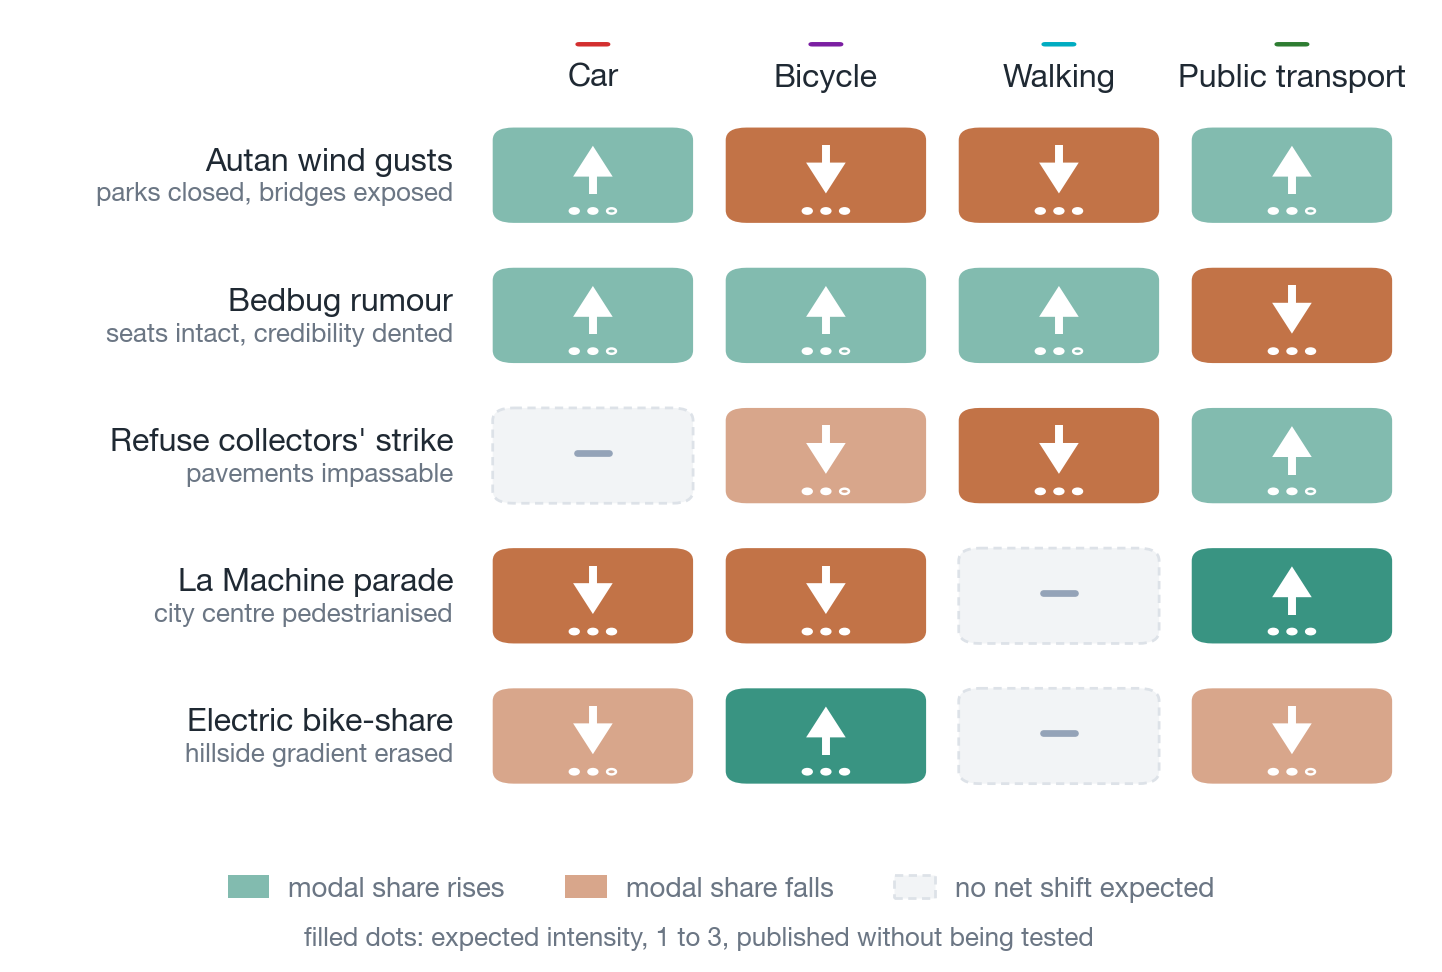
\includegraphics[width=0.95\columnwidth]{images/ch7_grille_signes.png}
  \caption{The twenty expected signs, five articles by four modes, pre-registered before simulation.}
  \label{fig-grille-signes}
\end{figure}

\begin{table*}[tp]
  \caption{Pre-registered 20-cell directional hypotheses and behavioral rationales (frozen 2026-09-21).}
  \label{tab-pre-registered-signs}
  \small
  \begin{tabularx}{\textwidth}{@{}llccL@{}}
    \toprule
    Event & Mode & Sign & Intensity & Theoretical Behavioral Rationale \\
    \midrule
    A09 (Windstorm) & Car & $+$ & $2$ & Passenger compartment shields travelers from wind noise and physical strain \\
    A09 (Windstorm) & Bicycle & $-$ & $3$ & Destabilizing gusts on bridges and mandatory closures of park bike paths \\
    A09 (Windstorm) & Walking & $-$ & $3$ & Airborne dust, falling branches, and detours along perimeter boulevards \\
    A09 (Windstorm) & Transit & $+$ & $2$ & Underground metro crosses the Garonne river fully sheltered from gales \\
    \midrule
    A13 (Bedbugs) & Car & $+$ & $2$ & Avoiding shared passenger cabins for non-mandatory personal travel \\
    A13 (Bedbugs) & Bicycle & $+$ & $2$ & Shifting toward an individual open-air mode perceived under direct control \\
    A13 (Bedbugs) & Walking & $+$ & $2$ & Extending pedestrian range to bypass upholstered public transit seating \\
    A13 (Bedbugs) & Transit & $-$ & $3$ & Technical service remains active but psychological modal credibility collapses \\
    \midrule
    A07 (Strike) & Car & $0$ & $0$ & Counteracting effects: localized street congestion repels drivers while detours demand cars \\
    A07 (Strike) & Bicycle & $-$ & $2$ & Broken glass, slippery street waste, and forced spillover into general traffic \\
    A07 (Strike) & Walking & $-$ & $3$ & Obstructed sidewalks, foul odours, and forced walking on roadways \\
    A07 (Strike) & Transit & $+$ & $2$ & Underground metro completely bypasses blocked street-level public space \\
    \midrule
    A18 (La Machine) & Car & $-$ & $3$ & Downtown core gridlocked and underground parking garages fully inaccessible \\
    A18 (La Machine) & Bicycle & $-$ & $3$ & Dense pedestrian crowds prevent safe cycling across thoroughfares \\
    A18 (La Machine) & Walking & $0$ & $0$ & Dual polarity: attracts leisurely onlookers but severely impedes hurried utilitarian pedestrians \\
    A18 (La Machine) & Transit & $+$ & $3$ & Sole mechanical option capable of approaching the pedestrianized festival zone \\
    \midrule
    A25 (VélôToulouse) & Car & $-$ & $2$ & Suburban commuters switch to electric cycling to avoid morning highway queues \\
    A25 (VélôToulouse) & Bicycle & $+$ & $3$ & Electric assistance removes physical fatigue and hillside topographic barriers \\
    A25 (VélôToulouse) & Walking & $0$ & $0$ & Ambiguous net impact: denser docking stations shorten trips while transfers lengthen walking \\
    A25 (VélôToulouse) & Transit & $-$ & $2$ & Direct modal competition with slow hillside feeder bus connections \\
    \bottomrule
  \end{tabularx}
\end{table*}

Before executing inference queries, we froze the expected direction and intensity of modal shifts. Table~\ref{tab-pre-registered-signs} records the 20 directional hypotheses pre-registered on 2026-09-21 (\texttt{grille\_signes.yaml}). The visual  net impact: denser docking stations shorten trips while transfers lengthen walking \\
    A25 (VélôToulouse) & Transit & $-$ & $2$ & Direct modal competition with slow hillside feeder bus connections \\
    \bottomrule
  \end{tabularx}
\end{table*}



\subsection{Longitudinal Extinction and Household Transmission}

\begin{figure}[tp]
  \centering
  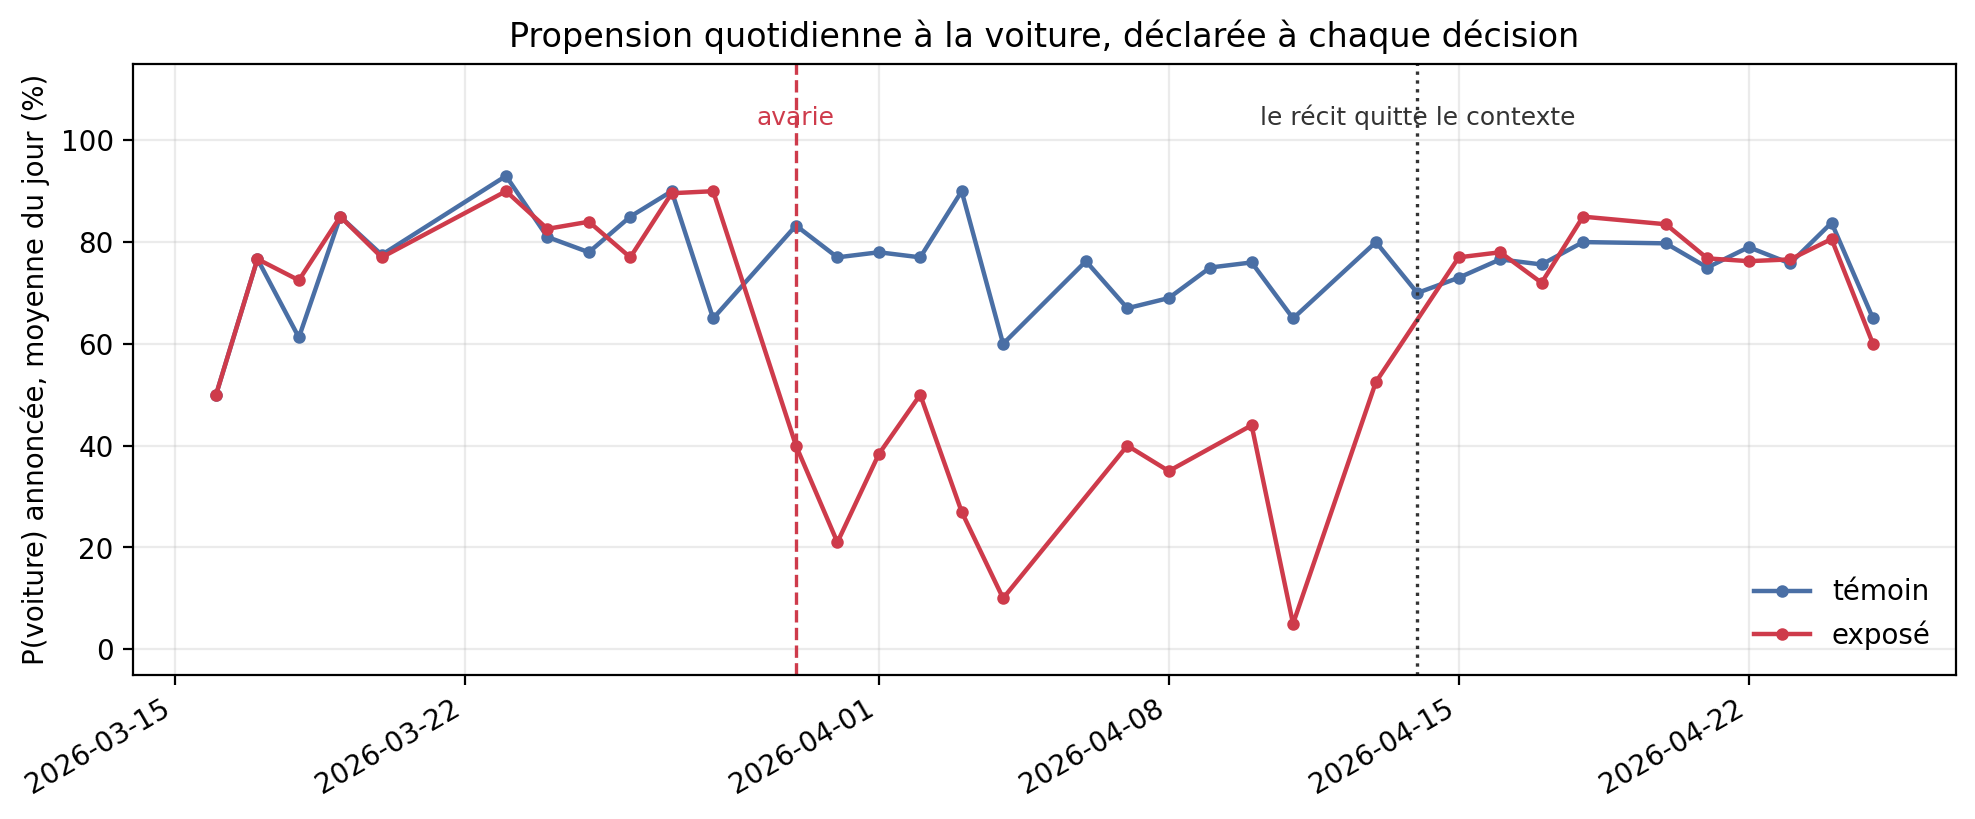
\includegraphics[width=0.95\columnwidth]{images/ch7_propension_quotidienne.png}
  \caption{Daily modal propensity towards private car following an unexpected incident.}
  \label{fig-propension}
\end{figure}

\begin{figure}[tp]
  \centering
  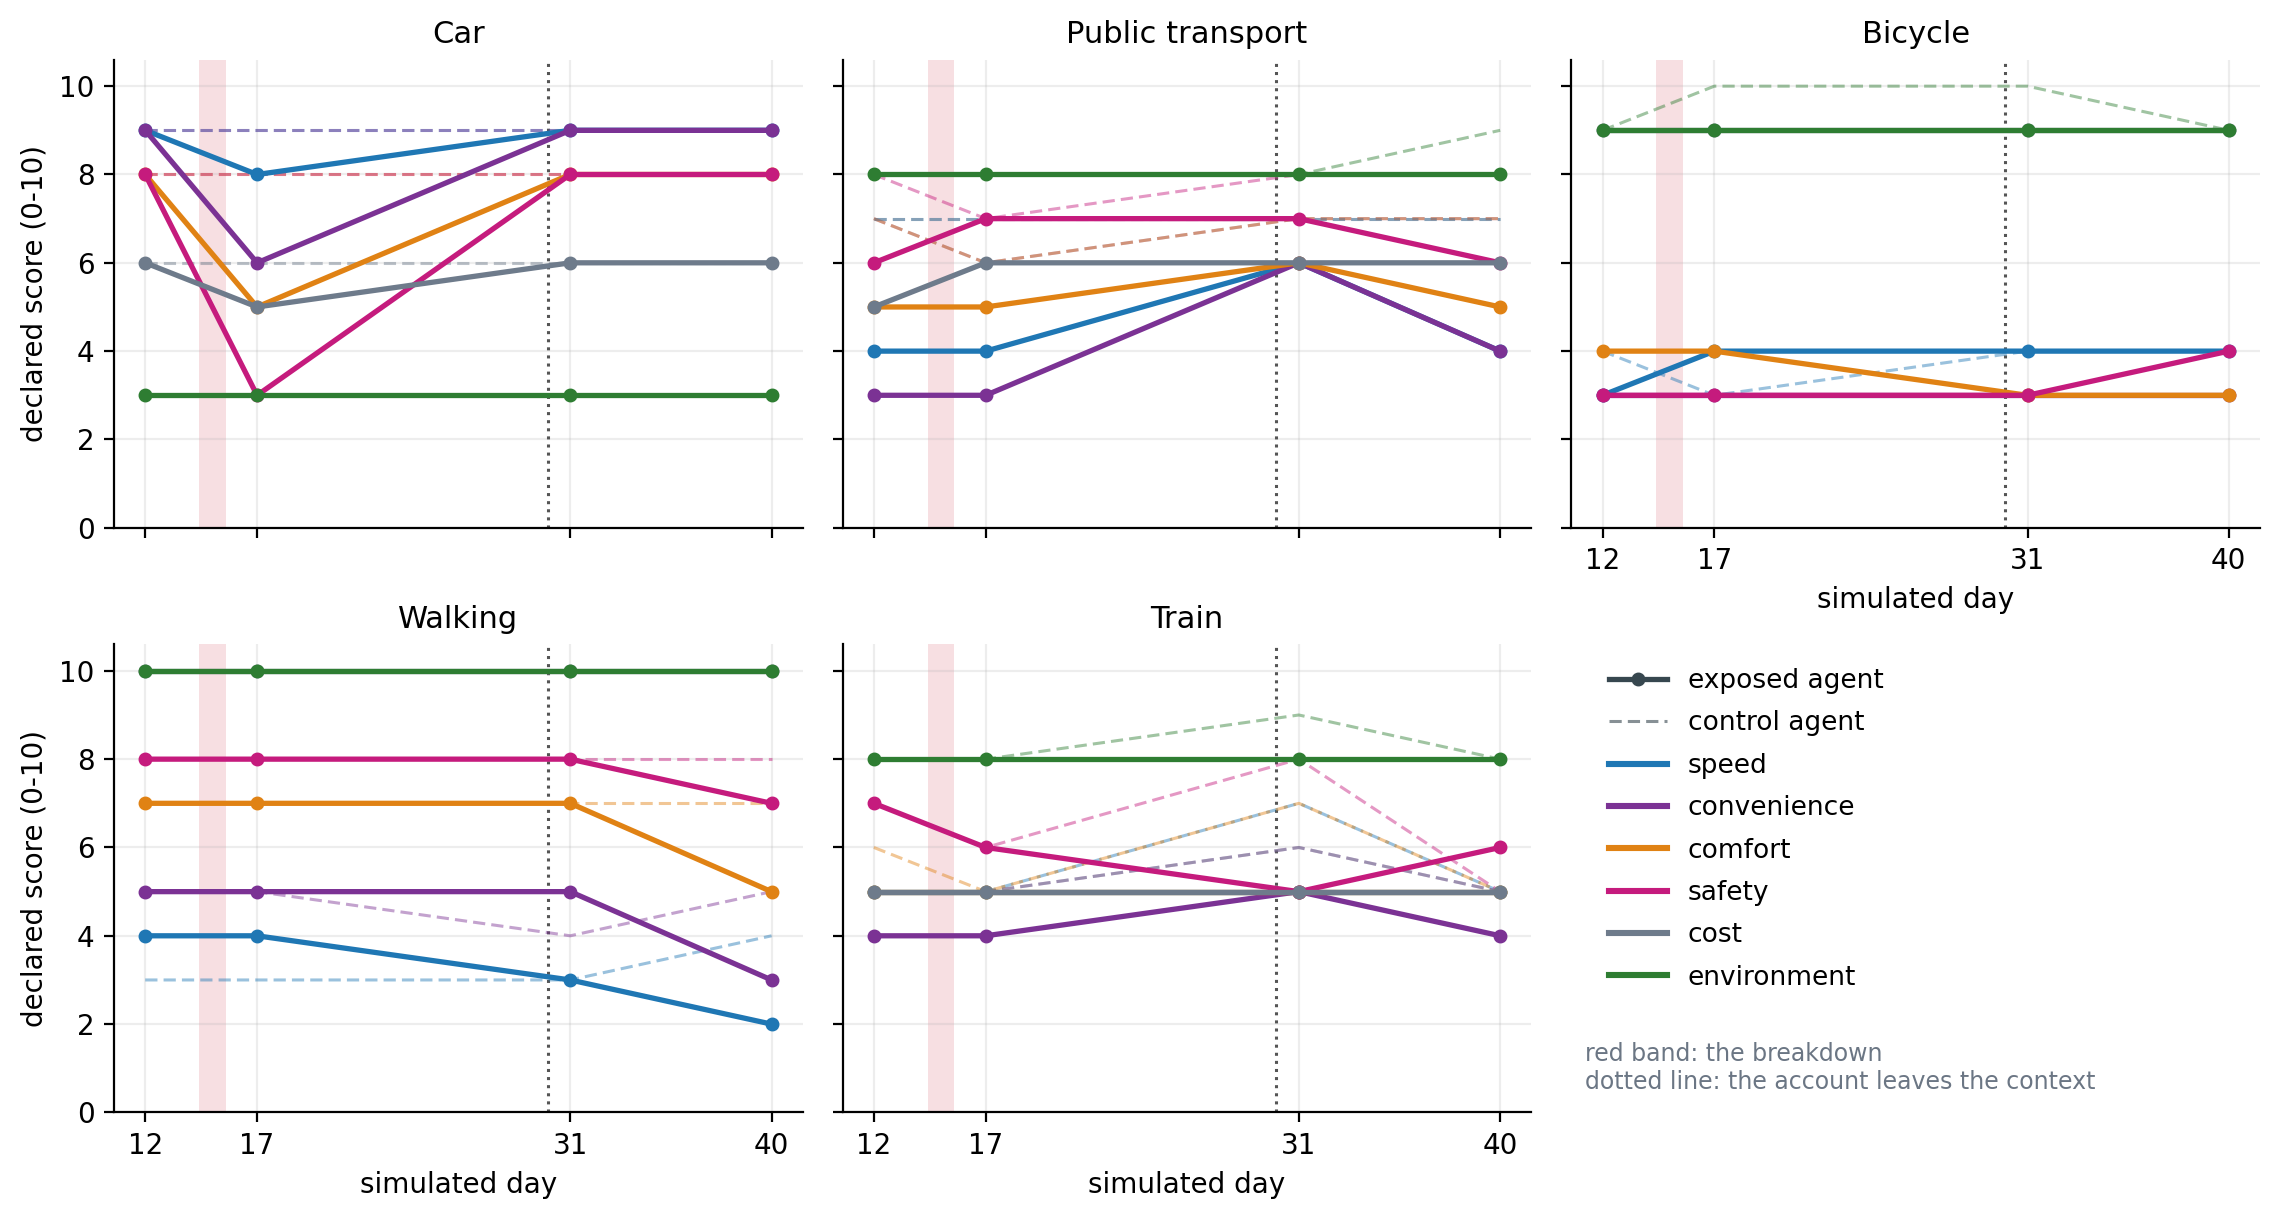
\includegraphics[width=0.95\columnwidth]{images/ch7_affinites_tous_modes.png}
  \caption{Declared multi-criteria affinities across modes, exposed vs control agent.}
  \label{fig-affinites}
\end{figure}

We track how shock perceptions propagate and extinguish over longitudinal multi-day runs. Figure~\ref{fig-propension} demonstrates the temporal trajectory of modal propensity following a disruption. Figure~\ref{fig-affinites} plots stated multi-criteria affinity ratings across four milestones.


\subsection{Pending Campaign Execution and Status}

\textbf{Pending Campaign Execution (\texttt{exp\_05a-e}).} The empirical execution of the five news shock campaigns across the synthetic cohort remains in progress. The final volume will incorporate empirical shift amplitudes, bootstrap confidence intervals, and directional sign concordance.
